% **************************** %
%          Slides GK           %
% **************************** %

\documentclass[10pt,fleqn]{beamer}
 
% **************************** %
%            Package           %
% **************************** %
% \usepackage{GarmirKhatch}
\usepackage[utf8]{inputenc}
\usepackage[T1]{fontenc}
\usepackage[french,english]{babel}
\usepackage[french]{layout}
\usepackage{lmodern}
\usepackage{ragged2e}
\usepackage{fancyhdr}
\usepackage{verbatim}
\usepackage{graphicx}
\usepackage{wrapfig}
\usepackage{url}
\usepackage{hyperref}
\usepackage{amsmath}
\usepackage{multirow}
\usepackage{multicol}
\usepackage{array}
\usepackage{colortbl}
\usepackage{comment}
\usepackage{tikz}
\usetikzlibrary{positioning, shadows}

\newcommand{\mo}{\textsc{Garmir~Khatch}}

% **************************** %
%          Préambule           %
% **************************** %
% Option pdf
\hypersetup{
      %pdfpagemode = FullScreen,
      pdfauthor   = {AMU FSI 2014},
      pdftitle    = {Présentation du projet TMS pour \mo},
      pdfsubject  = {Système de gestion des transports},
      pdfkeywords = {AMO, GK, TMS, CdC, DAT, PTI}
}
% Thème du pdf 
\usetheme{Warsaw}
% Logo de l'université d'Aix-Marseille
%\logo{\includegraphics[height=6mm]{logo}}
% Affiche les notes
%\setbeameroption{show notes}
% Blocks arrondies et ombrés
\setbeamertemplate{blocks}[rounded][shadow=true] 
% Balle pour la liste d'items
\setbeamertemplate{itemize item}[ball]
% Triangle pour la liste de sous items
\setbeamertemplate{itemize subitem}[triangle]
% Affiche l'ensemble du frame en gris clair
\beamertemplatetransparentcovered
% Faire apparaître un sommaire avant chaque section
\AtBeginSection[]{
	\begin{frame}
		\frametitle{Sommaire}
		\tableofcontents[currentsection, hideallsubsections]
	\end{frame}
}

% **************************** %
%        Page de garde         %
% **************************** %
\title[]{{\Large \textsc{\mo \\ Système de gestion des transports}}}
\author[\textsc{\mo - Système de gestion des transports}]{M2 FSIL - FSI}
\institute{Encadrant : M. Roland \textsc{Agopian}\\
Faculté des Sciences d'Aix-Marseille Université\\
Campus de Luminy}
\date{\scriptsize{ 27 mars 2014}}

% **************************** %
%       Corps du document      %
% **************************** %
\begin{document}
 
% **************************** %
%            Entête            %
% **************************** %
\begin{frame}
\begin{figure}
\centering

\includegraphics[scale=0.52]{Images/EnTeteSciences}
\end{figure}
\titlepage
\end{frame}

\begin{frame}
\frametitle{Sommaire}
\tableofcontents[hideallsubsections]
\end{frame}

\section[Mission d'AMO~: recueil des besoins (CdCF)]{Mission d'AMO~: recueil des besoins (CdCF)}

\subsection[Compréhension du contexte]{Compréhension du contexte}
\begin{frame}
\end{frame}

\subsection[Compréhension des besoins]{Compréhension des besoins}
\begin{frame}
\end{frame}

% ------------------------------------------------------------------------------
% ------------------------------------------------------------------------------
\subsection{Norme NF X50-151}

% ▿▿▿▿▿▿▿▿▿▿▿▿▿▿▿▿▿▿▿▿▿▿▿▿▿▿▿▿▿▿▿▿▿▿▿▿▿▿▿▿▿▿▿▿▿▿▿▿▿▿▿▿▿▿▿▿▿▿▿▿▿▿▿▿▿▿▿▿▿▿▿▿▿▿▿▿▿▿
\begin{frame}
\tableofcontents[subsectionstyle=show/shaded/hide, subsubsectionstyle=hide, sectionstyle=show/hide]
\end{frame}
% ▵▵▵▵▵▵▵▵▵▵▵▵▵▵▵▵▵▵▵▵▵▵▵▵▵▵▵▵▵▵▵▵▵▵▵▵▵▵▵▵▵▵▵▵▵▵▵▵▵▵▵▵▵▵▵▵▵▵▵▵▵▵▵▵▵▵▵▵▵▵▵▵▵▵▵▵▵▵

% ▿▿▿▿▿▿▿▿▿▿▿▿▿▿▿▿▿▿▿▿▿▿▿▿▿▿▿▿▿▿▿▿▿▿▿▿▿▿▿▿▿▿▿▿▿▿▿▿▿▿▿▿▿▿▿▿▿▿▿▿▿▿▿▿▿▿▿▿▿▿▿▿▿▿▿▿▿▿
\begin{frame}
\frametitle{Contenu (non exhaustif) de la norme NF X50-151}

\begin{block}{Pourquoi une norme ?}
\begin{itemize}
    \item Nous aider
    \item Être \og{}standard\fg{}
\end{itemize}

\end{block}
\end{frame}

\begin{frame}
\frametitle{Contenu (non exhaustif) de la norme NF X50-151}
\begin{exampleblock}{1/3 - Présentation du projet}
\begin{itemize}
    \item Le projet en lui même \small(finalités, retours sur investissements)
    \item Contexte \small(études réalisées, suites, nature des prestations, confidentialité)
    \item Énoncé du besoin \small(du point de vue de l'utillisateur)
    \item Environnement \small(utilisateurs, caractéristiques et contraintes matérielles)
\end{itemize}
\end{exampleblock}
\end{frame}

\begin{frame}
\frametitle{Contenu (non exhaustif) de la norme NF X50-151}
\begin{exampleblock}{2/3 - Expression fonctionnelle du besoin}
\begin{itemize}
    \item Fonctions principales (métier)
    \item Fonction complémentaires
    \item Critères d'appréciation de la solution fournie
\end{itemize}
\end{exampleblock}

\end{frame}
% ▵▵▵▵▵▵▵▵▵▵▵▵▵▵▵▵▵▵▵▵▵▵▵▵▵▵▵▵▵▵▵▵▵▵▵▵▵▵▵▵▵▵▵▵▵▵▵▵▵▵▵▵▵▵▵▵▵▵▵▵▵▵▵▵▵▵▵▵▵▵▵▵▵▵▵▵▵▵

% ▿▿▿▿▿▿▿▿▿▿▿▿▿▿▿▿▿▿▿▿▿▿▿▿▿▿▿▿▿▿▿▿▿▿▿▿▿▿▿▿▿▿▿▿▿▿▿▿▿▿▿▿▿▿▿▿▿▿▿▿▿▿▿▿▿▿▿▿▿▿▿▿▿▿▿▿▿▿
\begin{frame}
\frametitle{Contenu (non exhaustif) de la norme NF X50-151}
%\frametitle{Contenu (suite)}

\begin{exampleblock}{3/3 - Cadre de réponse}
Pour chaque fonction :
\begin{itemize}
    \item Description de la solution proposée
    \item Mise en évidence des critères d'appréciation
    \item Coût
\end{itemize}
Pour l'ensemble :
\begin{itemize}
    \item Écarts par rapport au CdCF
    \item Mesures prises pour respecter les contraintes
    \item Documentation technique \& utilisateur
    \item Modularité
    \item Fiabilité
    \item Évolutions technologiques
\end{itemize}
\end{exampleblock}

\end{frame} % Fin de la frame [Contenu (suite)]
% ▵▵▵▵▵▵▵▵▵▵▵▵▵▵▵▵▵▵▵▵▵▵▵▵▵▵▵▵▵▵▵▵▵▵▵▵▵▵▵▵▵▵▵▵▵▵▵▵▵▵▵▵▵▵▵▵▵▵▵▵▵▵▵▵▵▵▵▵▵▵▵▵▵▵▵▵▵▵

% Fin de la sous-section [Norme]
% ------------------------------------------------------------------------------

% ------------------------------------------------------------------------------

\section[Mission de maîtrise d'œuvre~: réalisation du projet]{Mission de maîtrise d'œuvre~: réalisation du projet}

% ------------------------------------------------------------------------------
%-------------------------------------------------------------------------------
%
%     CHARGEMENT DES EXTENSIONS
%
%-------------------------------------------------------------------------------

\documentclass[11pt,fleqn]{report}

\usepackage{garmirkhatch}



%-------------------------------------------------------------------------------
%
%     GLOBAL VALUES
%
%-------------------------------------------------------------------------------


%-------------------------------------------------------------------------------
%     Informations spécifiques au document
%-------------------------------------------------------------------------------

\ZTitle{Système de gestion des transports}
\ZSubject{Cahier des charges}
\ZVersion{2.0}
\ZDate{2014-03-03}
\ZAuthor{\Balde,\\\Cadon,\\\Gairoard,\\\Julien,\\\Lericolais,\\\Mezelle,\\\Pachy,\\\SuangaWeto,\\\Toure}


%-------------------------------------------------------------------------------
%     Contenu
%-------------------------------------------------------------------------------

\begin{document}

\ZMakeCover

\ZMakeInformations{
	% Historique des modifications
	% Version & Date & Auteur(s) & Modification(s)
	0.0 & 2014-03-03 & \Cadon & Création \\
}{
	% Historique des approbations
	% Version & Date & Approbateur(s)
	0.0 & 2014-03-03 & \Cadon \\
}{
	% Historique des validations
	% Version & Date & Responsable(s)
	0.0 & 2014-03-03 & \Cadon \\
}

\ZMakeTableOfContents

\chapter{Introduction}
Ce document présente le Plan d'Assurance Qualité (PAQ) relatif au projet de Transport Management System (TMS) par l'assistance à maîtrise d'ouvrage \amo au bénéfice de \mo.
\\
Il définit donc les méthodes, l'organisation et les éléments permettant d'assurer et de contrôler la qualité du projet.

\chapter{Structure du projet}
L'ensemble des documents produits durant le projet sera composé~:
\begin{enumerate}
	\item du PAQ~;
	\item du cahier des charges~;
	\item des comptes rendus de réunions~;
	\item des listes des tâches avec les assignations.
\end{enumerate}

\chapter{Organisation et suivi du projet}

\section{Acteurs}
\begin{table}[htbp]
	\begin{tabularx}{\linewidth}{X X}
		\toprule
		\textbf{Prénom(s) \& Nom} & \textbf{Adresse e-mail} \\
		\midrule
		\Agopian & \AgopianEmail \\
		\hline
		\Balde & \BaldeEmail \\
		\hline
		\Cadon & \CadonEmail \\
		\hline
		\Gairoard & \GairoardEmail \\
		\hline
		\Julien & \JulienEmail \\
		\hline
		\Lericolais & \LericolaisEmail \\
		\hline
		\Mezelle & \MezelleEmail \\
		\hline
		\Pachy & \PachyEmail \\
		\hline
		\SuangaWeto & \SuangaWetoEmail \\
		\hline
		\Toure & \ToureEmail \\
		\bottomrule
	\end{tabularx}
	\caption{Liste des acteurs}
	\label{Acteurs}
\end{table}

\section{Méthodologie de gestion du projet}
La méthodologie de gestion du projet de réalisation du TMS suit un cycle de développement en V, guidé par les tests et dont les principes sont~:
\begin{enumerate}
	\item tous les acteurs sont joignables par e-mail~;
	\item des réunions hebdomadaires externes sont planifiées jusqu'à la livraison finale tous les vendredis matins sur le campus universitaire de Saint-Charles à Marseille~;
	\item les présentations de l'avancement de l'application sont fréquentes et se déroulent pendant les réunions avec le représentant de la société.
\end{enumerate}
Afin de favoriser le partage des connaissances entre chaque membre du groupe, les différentes tâches seront effectuées principalement en binôme. La composition de chaque binôme variera en fonction des tâches à réaliser et des savoir-faire de chacun.
\\
Une fois qu'une tâche est terminée, si celle-ci a une suite logique, il incombe aux prédécesseurs de prévenir les successeurs.

\section{Réunions}

\subsection{Réunions internes}
Des réunions internes bihebdomadaires sont organisées afin de garantir une bonne coordination de l'équipe. Durant ces réunions tous les membres sont présents.

\subsection{Réunions externes}
Des réunions externes hebdomadaires sont organisées avec le représentant de la société afin de garantir une réactivité optimale concernant ses attentes et ses besoins.
\\
Les réunions externes donnent lieu à la rédaction d'un compte rendu contenant la liste exhaustive des tâches à réaliser, et remis au client au plus tard 48h après la fin de la réunion (dans les jours ouvrables).

\section{Outils de travail}
Afin d'éviter des problèmes d'incompatibilité, les outils suivants seront utilisés~:
\begin{table}[htbp]
	\centering
	\begin{tabularx}{\linewidth}{m{30mm} m{30mm} X}
		\toprule
		\textbf{Nom} & \textbf{Version} & \textbf{URL} \\
		\midrule
		GNU/Linux & Ubuntu 12.04 LTS & www.ubuntu.fr \\
		GNU/Linux & Debian & www.debian.org \\
		Microsoft~Windows & 7 & www.microsoft.com \\
		\bottomrule
	\end{tabularx}
	\caption{Outils de travail~: systèmes d'exploitation}
	\label{OutilsOS}
\end{table}
\begin{table}[htbp]
	\centering
	\begin{tabularx}{\linewidth}{m{30mm} m{30mm} X}
		\toprule
		\textbf{Nom} & \textbf{Version} & \textbf{URL} \\
		\midrule
		LaTeX & - & - \\
		\bottomrule
	\end{tabularx}
	\caption{Outils de travail~: documentation}
	\label{OutilsDocumentation}
\end{table}
\begin{table}[htbp]
	\centering
	\begin{tabularx}{\linewidth}{m{30mm} m{30mm} X}
		\toprule
		\textbf{Nom} & \textbf{Version} & \textbf{URL} \\
		\midrule
		Github & 1.7.9.5 & https://github.com/raviluminy/gk \\
		\bottomrule
	\end{tabularx}
	\caption{Outils de travail~: partage des fichiers}
	\label{OutilsDepot}
\end{table}

\chapter{Abréviations}
\begin{table}[htbp]
	\centering
	\begin{tabularx}{\linewidth}{m{30mm} X}
		\toprule
		\textbf{Abréviation} & \textbf{Signification} \\
		\midrule
		AMO & Assistance à Maîtrise d'Ouvrage \\
		CdC & Cahier des Charges \\
		CdCF & Cahier des Charges Fonctionnel \\
		CdCT & Cahier des Charges Technique \\
		CR & Compte-rendu \\
		Go & Giga-octet \\
		LdT & Liste des Tâches \\
		OdJ & Ordre du Jour \\
		PAQ & Plan d'Assurance Qualité \\
		SGBD & Système de Gestion de Bases de Données \\
		SGBDR & Système de Gestion de Bases de Données Relationnelles \\
		DAT & Dossier d'Architecture Technique \\
		PTI & Protocole Technique d'Installation \\
		PdR & Procédure de Recette \\
		DE & Dossier d'Exploitation \\
		PCS & Plan de Continuité des Services \\
		\bottomrule
	\end{tabularx}
	\caption{Abréviations communes}
	\label{AbreviationsCommunes}
\end{table}

\chapter{Gestion de la documentation}
Cette section décrit la manière dont sont gérés les documents relatifs au projet.

\section{Structure des documents}
Tout document produit doit se plier au modèle de document de la société.

\section{Nomenclature}
La liste exhaustive des documents concernés est décrite ci-dessous (hors sous-documents, images et librairies)~:
\begin{enumerate}
	\item \textbf{/Annexe/Docs/}
	\\
	Contient les documents relatifs à \mo, dont~:
	\begin{enumerate}
		\item GARMIR KHATCH - EXEMPLE DE CONTRAT DE TRANSPORT.doc,
		\item GARMIR KHATCH - SUIVI DES TRANSPORTS (EXEMPLE).xlsx,
		\item LOGISTICS REQUISITION.pdf,
		\item WAYBILL DELIVERY NOTE.pdf~;
	\end{enumerate}
	\item \textbf{/Annexe/RE/}
	\\
	Contient les documents relatifs aux réunions externes~:
	\begin{enumerate}
		\item RE-XXX-(YYYY-MM-DD)-CR-\textit{version}.tex,
		\item RE-XXX-(YYYY-MM-DD)-LdT-\textit{version}.tex,
		\item RE-XXX-(YYYY-MM-DD)-OdJ-\textit{version}.tex~;
	\end{enumerate}
	\item \textbf{/Annexe/RI/}
	\\
	Contient les documents relatifs aux réunions internes~:
	\begin{enumerate}
		\item RI-XXX-(YYYY-MM-DD)-CR-\textit{version}.tex,
		\item RI-XXX-(YYYY-MM-DD)-LdT-\textit{version}.tex,
		\item RI-XXX-(YYYY-MM-DD)-OdJ-\textit{version}.tex~;
	\end{enumerate}
	\item \textbf{/Conception/}
	\\
	Contient les documents relatifs à la conception~:
	\begin{enumerate}
		\item CdC-\textit{version}.tex,
		\item CdCF-\textit{version}.tex,
		\item CdCT-\textit{version}.tex,
		\item PAQ-\textit{version}.tex~;
	\end{enumerate}
	\item \textbf{/Realisation/}
	\\
	Contient les documents relatifs à la réalisation~:
	\begin{enumerate}
		\item DAT-\textit{version}.tex,
		\item PTI-\textit{version}.tex,
		\item PdR-\textit{version}.tex,
		\item DE-\textit{version}.tex,
		\item PCS-\textit{version}.tex.
	\end{enumerate}
\end{enumerate}
Dans chaque document énoncé, l'élément \textit{version} représente la version du fichier dans un format pointé. Ci-dessous quelques exemples~:
\begin{enumerate}
	\item /Annexe/RE/RE-001-(2014-02-07)-CR-2.0.tex~;
	\item /Annexe/RI/RI-003-(2014-02-21)-OdJ-1.3.tex~;
	\item /Conception/CdCF-2.1.tex~;
	\item /Realisation/DAT-0.1.tex.
\end{enumerate}

\chapter{Planification}

\begin{figure}
	\centering
	\begin{tikzpicture}
		% Déclaration des styles
		\tikzstyle{tache}=[rectangle,text=black,minimum height=9mm,minimum width=19mm]
		\tikzstyle{temps}=[rectangle,text=black,minimum height=9mm,minimum width=9mm]
		\tikzstyle{jour}=[rectangle,text=black,minimum height=9mm,minimum width=13mm,draw=black,fill=black!5]
		\tikzstyle{color1}=[draw=ZMainColor,fill=black!5]
		\tikzstyle{color2}=[draw=red,       fill=red!5]
		\tikzstyle{color3}=[draw=green,     fill=green!5]
		\tikzstyle{color4}=[draw=orange,    fill=orange!5]
		\tikzstyle{color5}=[draw=blue,      fill=blue!5]
		\tikzstyle{color6}=[draw=magenta,   fill=magenta!5]
		% Déclaration des noeuds
		% Déclaration des noeuds de temps
		\node[jour] (j1) at ( 30mm, 15mm) {\centering\tiny Vendredi};
		\node[jour] (j2) at ( 44mm, 15mm) {\centering\tiny Samedi};
		\node[jour] (j3) at ( 58mm, 15mm) {\centering\tiny Dimanche};
		\node[jour] (j4) at ( 72mm, 15mm) {\centering\tiny Lundi};
		\node[jour] (j5) at ( 86mm, 15mm) {\centering\tiny Mardi};
		\node[jour] (j6) at (100mm, 15mm) {\centering\tiny Mercredi};
		\node[jour] (j7) at (114mm, 15mm) {\centering\tiny Jeudi};
		% Déclaration des noeuds de tâches
		\node[tache,color1] (t1) at ( 0mm,- 0mm) {Tâche1};
		\node[temps,color1] (h1) at (15mm,- 0mm) {Xh};
		\node[tache,color2] (t2) at ( 0mm,-10mm) {Tâche2};
		\node[temps,color2] (h2) at (15mm,-10mm) {Xh};
		\node[tache,color3] (t3) at ( 0mm,-20mm) {Tâche3};
		\node[temps,color3] (h3) at (15mm,-20mm) {Xh};
		\node[tache,color4] (t4) at ( 0mm,-30mm) {Tâche4};
		\node[temps,color4] (h4) at (15mm,-30mm) {Xh};
		\node[tache,color5] (t5) at ( 0mm,-40mm) {Tâche5};
		\node[temps,color5] (h5) at (15mm,-40mm) {Xh};
		\node[tache,color6] (t6) at ( 0mm,-50mm) {Tâche6};
		\node[temps,color6] (h6) at (15mm,-50mm) {Xh};
		% Déclaration des lignes de tâches
		\draw[color1] (h1) -- (120mm,- 0mm);
		\draw[color2] (h2) -- (120mm,-10mm);
		\draw[color3] (h3) -- (120mm,-20mm);
		\draw[color4] (h4) -- (120mm,-30mm);
		\draw[color5] (h5) -- (120mm,-40mm);
		\draw[color6] (h6) -- (120mm,-50mm);
		% Déclaration des noeuds d'affectation
		\node[tache,color1] (a1) at (60mm,- 0mm) {Ressources1};
		\node[tache,color2] (a2) at (60mm,-10mm) {Ressources2};
		\node[tache,color3] (a3) at (60mm,-20mm) {Ressources3};
		\node[tache,color4] (a4) at (60mm,-30mm) {Ressources4};
		\node[tache,color5] (a5) at (60mm,-40mm) {Ressources5};
		\node[tache,color6] (a6) at (60mm,-50mm) {Ressources6};
	\end{tikzpicture}
	\caption{Planification}
	\label{Planification}
\end{figure}

\end{document}

% ------------------------------------------------------------------------------
\subsection[Réponse technique aux besoins fonctionnels (DAT)]{Réponse technique aux besoins fonctionnels (DAT)}
\begin{frame}
\frametitle{}
\begin{block}{\textbf{Qu'est-ce que \mo~?}}
\begin{itemize}
\item Organisation humanitaires (187 Sociétés Nationales)
\item Vient en aide aux personnes plus vulnérables
\item Fort réseau de volontaires
\item Rend les communautés plus résistantes
\end{itemize}
\end{block}
\end{frame}
% ------------------------------------------------------------------------------
% ------------------------------------------------------------------------------
\subsection{Synchronisation}

% ▿▿▿▿▿▿▿▿▿▿▿▿▿▿▿▿▿▿▿▿▿▿▿▿▿▿▿▿▿▿▿▿▿▿▿▿▿▿▿▿▿▿▿▿▿▿▿▿▿▿▿▿▿▿▿▿▿▿▿▿▿▿▿▿▿▿▿▿▿▿▿▿▿▿▿▿▿▿
\begin{frame}
\tableofcontents[subsectionstyle=show/shaded/hide, subsubsectionstyle=hide, sectionstyle=show/hide]
\end{frame}
% ▵▵▵▵▵▵▵▵▵▵▵▵▵▵▵▵▵▵▵▵▵▵▵▵▵▵▵▵▵▵▵▵▵▵▵▵▵▵▵▵▵▵▵▵▵▵▵▵▵▵▵▵▵▵▵▵▵▵▵▵▵▵▵▵▵▵▵▵▵▵▵▵▵▵▵▵▵▵

% ▿▿▿▿▿▿▿▿▿▿▿▿▿▿▿▿▿▿▿▿▿▿▿▿▿▿▿▿▿▿▿▿▿▿▿▿▿▿▿▿▿▿▿▿▿▿▿▿▿▿▿▿▿▿▿▿▿▿▿▿▿▿▿▿▿▿▿▿▿▿▿▿▿▿▿▿▿▿
\begin{frame}
\frametitle{Introduction}

\begin{block}{Contexte}
\begin{itemize}
    \item Liaison réseau pas toujours accessible
    \item Plusieurs utilisateurs peuvent modifier la même donnée
\end{itemize}
\end{block}

\pause

\begin{exampleblock}{Idée}
\begin{itemize}
    \item Gérer deux modes~: Connecté (synchrone), Hors-ligne (asynchrone)
    \item Logger tout ajout ou modification (avec horodatage)
    \item S'en servir pour la fusion
\end{itemize}
\end{exampleblock}

\pause

\begin{alertblock}{Problématique}
\begin{itemize}
    \item Cohérence des données
    \item Conflits
\end{itemize}
\end{alertblock}

\end{frame} % Fin de la frame [Introduction]
% ▵▵▵▵▵▵▵▵▵▵▵▵▵▵▵▵▵▵▵▵▵▵▵▵▵▵▵▵▵▵▵▵▵▵▵▵▵▵▵▵▵▵▵▵▵▵▵▵▵▵▵▵▵▵▵▵▵▵▵▵▵▵▵▵▵▵▵▵▵▵▵▵▵▵▵▵▵▵

% ▿▿▿▿▿▿▿▿▿▿▿▿▿▿▿▿▿▿▿▿▿▿▿▿▿▿▿▿▿▿▿▿▿▿▿▿▿▿▿▿▿▿▿▿▿▿▿▿▿▿▿▿▿▿▿▿▿▿▿▿▿▿▿▿▿▿▿▿▿▿▿▿▿▿▿▿▿▿
\begin{frame}
\frametitle{Modes de connexion}
\begin{figure}[htbp]
    \centering
    \scalebox{0.6}{
	    \begin{tikzpicture}
	        % Styles :
		    \tikzstyle{titre}=[rectangle,draw,fill=white,text=black]
		    \tikzstyle{symbole}=[rectangle,text=black, scale=4]
		    \tikzstyle{serveurloc}=[rectangle,draw,fill=blue!50,text=white, minimum height=2cm]
		    \tikzstyle{serveurcen}=[rectangle,draw,fill=yellow!50,text=black, minimum height=2cm]
	        % #### CADRE ROUGE :
		    % Fond :
		    \draw[fill=red!10] (0,0) rectangle (13, 4);
		    % Titres :
		    \node[titre] at (6.50,4.00) {Mode hors-ligne};
		    % Serveurs :
		    \node[serveurloc] at (6.00,2) {Serveur local};
		    \node[serveurcen] at (11.00,2) {Serveur central};
		    \node[symbole] at (8.50,2) {?};
		    \node[symbole] at (3.00,2) {X};
		    % Traits :
		    \draw[line width=2pt] (2, 2) -- (4, 2);
		    \draw[line width=2pt] (7.5, 2) -- (9.5, 2);
		    % Utilisateurs :
		    \umlactor[x=1.00, y=2.00]{Utilisateur}
		    % #### CADRE VERT :
		    % Fond :
		    \draw[fill=green!10] (0,5) rectangle (13, 9);
		    % Titres :
		    \node[titre] at (6.50,9.00) {Mode connecté};
		    % Serveurs :
		    \node[serveurloc] at (6.00,7) {Serveur local};
		    \node[serveurcen] at (11.00,7) {Serveur central};
		    \node[symbole] at (8.50, 7) {?};
		    % Traits :
		    \draw[line width=2pt] (2, 7) -- (4, 7);
		    \draw[line width=2pt] (7.5, 7) -- (9.5, 7);
		    % Utilisateurs :
		    \umlactor[x=1.00, y=7]{Utilisateur}
	    \end{tikzpicture}
    }
	\caption{Topologie des modes connecté et hors-ligne}
	\label{explicationcodeco}
\end{figure}
\end{frame} % Fin de la frame [Synchronisation]
% ▵▵▵▵▵▵▵▵▵▵▵▵▵▵▵▵▵▵▵▵▵▵▵▵▵▵▵▵▵▵▵▵▵▵▵▵▵▵▵▵▵▵▵▵▵▵▵▵▵▵▵▵▵▵▵▵▵▵▵▵▵▵▵▵▵▵▵▵▵▵▵▵▵▵▵▵▵▵

% ▿▿▿▿▿▿▿▿▿▿▿▿▿▿▿▿▿▿▿▿▿▿▿▿▿▿▿▿▿▿▿▿▿▿▿▿▿▿▿▿▿▿▿▿▿▿▿▿▿▿▿▿▿▿▿▿▿▿▿▿▿▿▿▿▿▿▿▿▿▿▿▿▿▿▿▿▿▿
\begin{frame}
\frametitle{Ajout / Modification de donnée}

En simplifié :

\begin{block}{Mode hors-ligne}
\begin{enumerate}
%\setcounter{enumi}{}
    \item Demande d'ajout/modification de l'utilisateur
\end{enumerate}
\vspace{-1em}
\hspace*{.05\linewidth}\begin{minipage}{.9\linewidth}
\begin{exampleblock}{Mode connecté uniquement}
\begin{enumerate}
    \setcounter{enumi}{1}
    \item Demande de permission au serveur
    \item Envoi de l'ajout/modification
    \item Attente de confirmation
\end{enumerate}
\end{exampleblock}
\end{minipage}
\begin{enumerate}
\setcounter{enumi}{4}
    \item (Ssi première \emph{modification} :) \textbf{log} de la donnée originelle
    \item Application des changements en local
    \item \textbf{Log} des détails du changement
\end{enumerate}
\end{block}


\end{frame} % Fin de la frame [Ajout / Modification en mode connecté]
% ▵▵▵▵▵▵▵▵▵▵▵▵▵▵▵▵▵▵▵▵▵▵▵▵▵▵▵▵▵▵▵▵▵▵▵▵▵▵▵▵▵▵▵▵▵▵▵▵▵▵▵▵▵▵▵▵▵▵▵▵▵▵▵▵▵▵▵▵▵▵▵▵▵▵▵▵▵▵

% ▿▿▿▿▿▿▿▿▿▿▿▿▿▿▿▿▿▿▿▿▿▿▿▿▿▿▿▿▿▿▿▿▿▿▿▿▿▿▿▿▿▿▿▿▿▿▿▿▿▿▿▿▿▿▿▿▿▿▿▿▿▿▿▿▿▿▿▿▿▿▿▿▿▿▿▿▿▿
\begin{frame}
\frametitle{Synchronisation}

\begin{block}{Étapes}
\begin{enumerate}
    %\setcounter{enumi}{}
    \item Envoi de la date courrante au serveur % Pour pouvoir calculer les éventuels écarts entre la date client et la date serveur
    \item Récupération des logs ultérieurs à la dernière synchronisation
\end{enumerate}
\vspace{-1em}
\hspace*{.05\linewidth}\begin{minipage}{.9\linewidth}
    \begin{block}{Pour chaque donnée modifiée localement :}
    \begin{enumerate}
    \setcounter{enumi}{2}
        \item Vérification des droits
        \item Si conflit : Choix de l'utilisateur entre la donnée locale et la serveur (en fonction de l'originale)
    \end{enumerate}
    \end{block}
\end{minipage}
\begin{enumerate}
\setcounter{enumi}{4}
    \item Application des changements en local
    \item Génération d'\textbf{un} log global des modifications
    \item Envoi au serveur
    \item Attente de confirmation
    \item MAJ de la date de la dernière synchronisation
\end{enumerate}
\end{block} 

\end{frame} % Fin de la frame [Synchronisation]
% ▵▵▵▵▵▵▵▵▵▵▵▵▵▵▵▵▵▵▵▵▵▵▵▵▵▵▵▵▵▵▵▵▵▵▵▵▵▵▵▵▵▵▵▵▵▵▵▵▵▵▵▵▵▵▵▵▵▵▵▵▵▵▵▵▵▵▵▵▵▵▵▵▵▵▵▵▵▵

% ▿▿▿▿▿▿▿▿▿▿▿▿▿▿▿▿▿▿▿▿▿▿▿▿▿▿▿▿▿▿▿▿▿▿▿▿▿▿▿▿▿▿▿▿▿▿▿▿▿▿▿▿▿▿▿▿▿▿▿▿▿▿▿▿▿▿▿▿▿▿▿▿▿▿▿▿▿▿
\begin{frame}
\frametitle{Trafic réseau}

\begin{block}{Communications restreintes}
    \begin{itemize}
        \item GSM ou Satellitaire
        \item Débits faibles
    \end{itemize}
\end{block}

\begin{exampleblock}{Contre-mesures}
\begin{itemize}
    \item Choix des éléments synchronisables
    \item Log unique pour l'ajout/modification (synchronisation)
\end{itemize}
\end{exampleblock}

\end{frame} % Fin de la frame [Gestion du trafic réseau]
% ▵▵▵▵▵▵▵▵▵▵▵▵▵▵▵▵▵▵▵▵▵▵▵▵▵▵▵▵▵▵▵▵▵▵▵▵▵▵▵▵▵▵▵▵▵▵▵▵▵▵▵▵▵▵▵▵▵▵▵▵▵▵▵▵▵▵▵▵▵▵▵▵▵▵▵▵▵▵

% Fin de la sous-section [Synchronisation]
% ------------------------------------------------------------------------------

% ▿▿▿▿▿▿▿▿▿▿▿▿▿▿▿▿▿▿▿▿▿▿▿▿▿▿▿▿▿▿▿▿▿▿▿▿▿▿▿▿▿▿▿▿▿▿▿▿▿▿▿▿▿▿▿▿▿▿▿▿▿▿▿▿▿▿▿▿▿▿▿▿▿▿▿▿▿▿
% ▵▵▵▵▵▵▵▵▵▵▵▵▵▵▵▵▵▵▵▵▵▵▵▵▵▵▵▵▵▵▵▵▵▵▵▵▵▵▵▵▵▵▵▵▵▵▵▵▵▵▵▵▵▵▵▵▵▵▵▵▵▵▵▵▵▵▵▵▵▵▵▵▵▵▵▵▵▵

% ------------------------------------------------------------------------------

\subsection[Authentification et contrôle d'accès (LDAP)]{Authentification et contrôle d'accès (LDAP)}
\begin{frame}
  \frametitle{Authentification et contrôle d'accès}
  \begin{block}{\textbf{ Sommaire }}
  \begin{itemize}
  \item Les choix
  \item Architecture
  \item Gestion des droits
  \item Les Protocoles
  \item Réalisation
  \end{itemize}
  \end{block}
\end{frame}

\begin{frame}
  \frametitle{Authentification et contrôle d'accès : Les choix}
  \begin{block}{\textbf{Pourquoi un annuaire ? }}
  \begin{itemize}
  \item Plus consulté que mis à jour
  \item Structure hierachique 
  \end{itemize} 
  \end{block}
  
  \begin{block}{\textbf{Pourquoi LDAP ? }}
  \begin{itemize}
  \item Protocole réseau léger -> \textbf{Optimisation des flux
}
  \item Authentification et contrôle d'accès -> \textbf{Sécurité}
  \item Haute disponibilité via réplication  -> \textbf{Sécurité}
  \item Mécanisme de référencement
  \end{itemize}
  \end{block}
\end{frame}

  \frametitle{Authentification et contrôle d'accès}
  \begin{figure}[htbp]
	  \centering
	  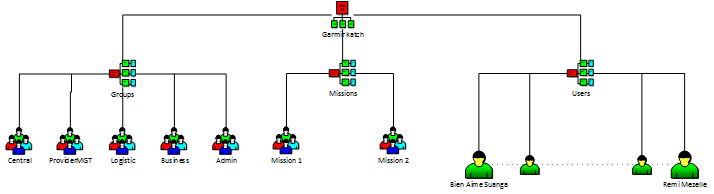
\includegraphics[scale=0.4]{Images/SchemaLDAP.png}
	  \caption{Structure de l'annuaire}
	  \label{SchemaLDAP}
  \end{figure}
 
  \begin{figure}[htbp]
	\centering
	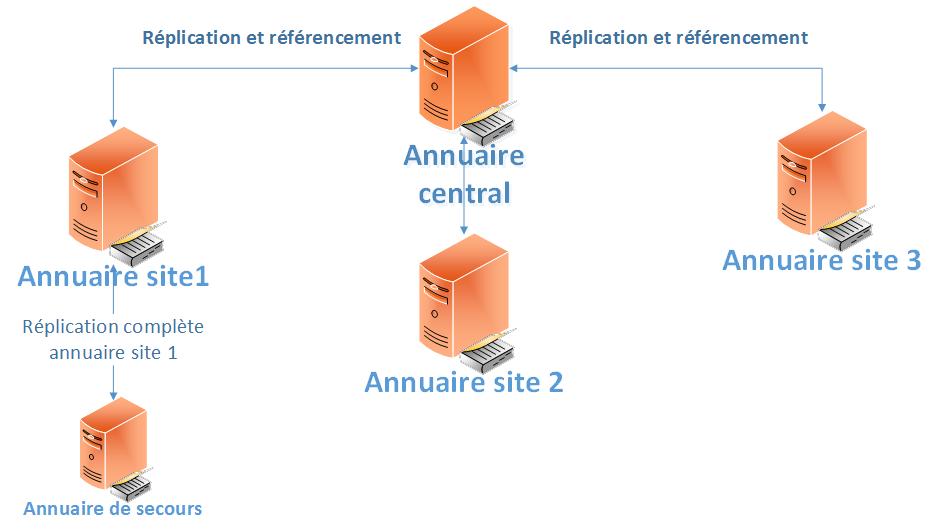
\includegraphics[scale=0.4]{Images/SchemaGlobal.png}
	\caption{Architecture globale}
	\label{SchemaGlobal}
\end{figure}

\begin{figure}[htbp]
	\centering
	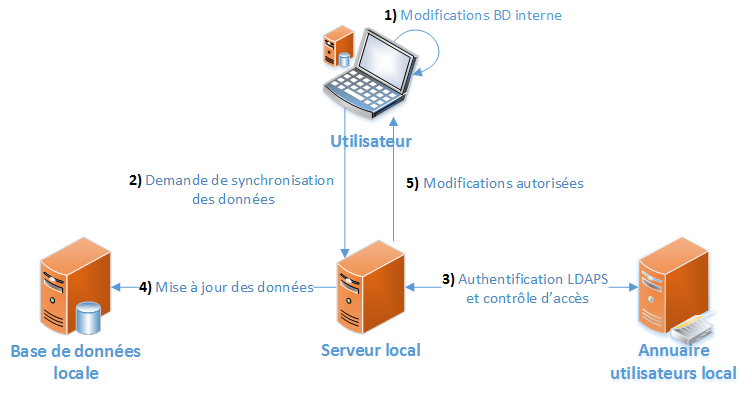
\includegraphics[scale=0.55]{Images/SchemaAuthentification.png}
	\caption{Authentification pour la synchronisation}
	\label{SchemaAuthentification}
\end{figure}

\begin{frame}
  \frametitle{Authentification et contrôle d'accès}
  \begin{block}{\textbf{Droits utilisateurs}}
  \begin{itemize}
  \item Droits pour chaque utilisateur
  \item Droits pour chaque groupe
  \item Autorisations et/ou refus
  \end{itemize}
  \end{block}
\end{frame}

\begin{frame}
  \frametitle{Authentification et contrôle d'accès}
  \begin{block}{\textbf{Gestion des droits}}
  \begin{itemize}
  \item Priorité aux droits directement liés à l'utilisateur 
  \item Priorité aux droits autorisés si l'utilisateur est lié à plusieurs groupes
  \item les droits du groupe
  \end{itemize}
  \end{block}
\end{frame}

\begin{frame}
  \frametitle{Authentification et contrôle d'accès}
  \begin{block}{\textbf{Autres Protocoles connus}}
  \begin{itemize}
  \item RADIUS (Remote Authentication Dial-In User Service)
  \item PAP (Password Authentication Protocol)
  \item MS-CHAP (Microsoft Challenge Handshake Authentication Protocol)
  \item ... 
  \end{itemize}
  \end{block}
%   Utiles si on sait comment se defendre face à une question
%   \begin{block}{\textbf{Quelques normes utiles}}
%   \begin{itemize}
%   \item X500 
%   \item UDDI : Universal Description Discovery and Integration
%   \item TULLEB : Titre Uniforme Labellisé Librement et Édité(Norme destinée aux annuaires publicitaires)
%   \item ... 
%   \end{itemize}
%   \end{block}
\end{frame}

\begin{frame}
  \frametitle{Authentification et contrôle d'accès}
  \begin{block}{\textbf{Travail effectué}}
  \begin{itemize}
  \item Mis en place du serveur 
    \begin{itemize}
    \item Windows
    \item Linux
    \end{itemize}
  \item Ajout d'un schema 
  \item Librairie de consulation via l'outil % à rénomer 
  \end{itemize}
  \end{block}
\end{frame}

\begin{frame}
  \frametitle{Authentification et contrôle d'accès}
  \begin{block}{\textbf{ce qu'il reste à faire}}
  \begin{itemize}
  \item Système de réplication et de référencement 
  \item Ajout et modification dans l'outil
  \end{itemize}
  \end{block}
\end{frame}

\begin{frame}
  \frametitle{Authentification et contrôle d'accès}
  \begin{block}{\textbf{Probleme rencontré }}
  \begin{itemize}
  \item Peu de connaissance de l'architecture LDAP
  \item Recherche des librairies LDAP pour windows 
  \item 
  \end{itemize}
  \end{block}
\end{frame}


\subsection[Tests sur l'interface graphique et unitaires (CdR)]{Tests sur l'interface graphique et unitaires (CdR)}
\begin{frame}
\frametitle{Les tests}
\begin{block}{\textbf{Pourquoi les tests sont importants dans ce projet}}
\begin{itemize}
\item l'outil doit être fiable
\item les fonctionnalités du cahier des charges doivent être opérationnelles
\end{itemize}
\end{block}
\end{frame}

\begin{frame}
\frametitle{}
\begin{block}{\textbf{Différents types de tests ont été réalisé : }}
\begin{itemize}
\item les tests sur l'interface graphique,
\item les tests unitaires,
\item les tests sur le système de gestion de données.
\end{itemize}
\end{block}
\begin{block}{\textbf{Configuration des tests : }}
\begin{itemize}
\item le framework Qt intègre une librairie de test : QTestlib
\item les tests sont lancés à partir de l'éxecutable
\item différentes options permettent de lancer les différents tests ( \emph{-testldap} )
\end{itemize}
\end{block}
\end{frame}

\begin{block}{\textbf{Test d'un champ sur l'onglet Réquisition }}
\begin{center}
\newcolumntype{R}[1]{>{\raggedleft\arraybackslash }b{#1}}
\newcolumntype{L}[1]{>{\raggedright\arraybackslash }b{#1}}
\newcolumntype{C}[1]{>{\centering\arraybackslash }b{#1}}
\begin{tabular}{|L{2.7cm}|L{7cm}|}
\hline \emph{Cas de test :} & Test-Graphique-08  \\
\hline \emph{Titre :} & testCountryCode   \\
\hline \emph{Objectif :} & Vérifier le bon fonctionnement du champ du code pays dans l'onglet réquisition   \\
\hline \emph{Procédure :} & Cliquer dans le champ du code pays, le remplir avec une chaîne et vérifier que la chaîne correspond   \\
\hline \emph{Données de test :} & On rempli avec la chaîne ``Fr''   \\
\hline \emph{Config :} & Using QtTest library 5.2.1, Qt 5.2.1   \\
\hline \emph{Résultat :} & PASS   \\
\hline 
\end{tabular} 
\end{center}
\end{block} 

\begin{frame}
\begin{block}{\textbf{Les tests graphiques permettent de }}
\begin{itemize}
\item tester les zones de saisies
\item tester les validateurs
\end{itemize}
\end{block}
\end{frame}

\begin{block}{\textbf{Test d'un champ sur l'onglet Providers }}
\begin{center}
\newcolumntype{R}[1]{>{\raggedleft\arraybackslash }b{#1}}
\newcolumntype{L}[1]{>{\raggedright\arraybackslash }b{#1}}
\newcolumntype{C}[1]{>{\centering\arraybackslash }b{#1}}
\begin{tabular}{|L{2.7cm}|L{7cm}|}
\hline \emph{Cas de test :} & Test-Graphique-31  \\
\hline \emph{Titre :} & testWaybillCountryCode   \\
\hline \emph{Objectif :} & Vérifier le bon fonctionnement du champ du code pays du prestataire.   \\
\hline \emph{Procédure :} & Cliquer dans le champ, le remplir avec une chaîne et vérifier que la chaîne correspond   \\
\hline \emph{Données de test :} & On rempli avec la chaîne ``FRA''   \\
\hline \emph{Config :} & Using QtTest library 5.2.1, Qt 5.2.1   \\
\hline \emph{Résultat :} & PASS   \\
\hline 
\end{tabular} 
\end{center}
\end{block}

\begin{frame}
\begin{block}{\textbf{Les tests unitaires de l'annuaire LDAP permettent de}}
\begin{itemize}
\item tester les connexions au serveur
\item tester l'authentification
\item vérifier l'implémentation des groupes
\item tester les droits en\begin{itemize} \item lecture
					  \item écriture
					  \item ajout
					  \item suppression
			  \end{itemize}		
\end{itemize}
\end{block}
\end{frame}

\begin{block}{\textbf{Test d'une connexion à l'annuaire }}
\begin{center}
\newcolumntype{R}[1]{>{\raggedleft\arraybackslash }b{#1}}
\newcolumntype{L}[1]{>{\raggedright\arraybackslash }b{#1}}
\newcolumntype{C}[1]{>{\centering\arraybackslash }b{#1}}
\begin{tabular}{|L{2.7cm}|L{7cm}|}
\hline \emph{Cas de test :} & Test-Unitaire-01  \\
\hline \emph{Titre :} & testConnection   \\
\hline \emph{Objectif :} & Vérifier une connexion à l'annuaire LDAP   \\
\hline \emph{Procédure :} & Initialisation d'une connexion avec un nom d'hôte et un port existant   \\
\hline \emph{Données de test :} & hostname : localhost, port : 389   \\
\hline \emph{Résultat :} & PASS   \\
\hline 
\hline \emph{Cas de test :} & Test-Unitaire-02  \\
\hline \emph{Titre :} & testConnectionBadHostname   \\
\hline \emph{Objectif :} & Vérifier une connexion à l'annuaire LDAP   \\
\hline \emph{Procédure :} & Initialisation d'une connexion avec un faux nom d'hôte et un port existant   \\
\hline \emph{Données de test :} & hostname : toto, port : 389   \\
\hline \emph{Résultat :} & FAIL comme prévu   \\
\hline 
\end{tabular} 
\end{center}
\end{block}

\begin{frame}
\begin{block}{\textbf{Tous les tests sont visualisables dans le cahier des recettes}}
\end{block}
\end{frame}




\subsection[Procédure de déploiement et d'installation (PIT)]{Procédure de déploiement et d'installation (PIT)}
\begin{frame}
\end{frame}

\section[Conclusion]{Conclusion}

\subsection[Conclusion]{Conclusion}
\begin{frame}
	\transdissolve[duration=0.2]<1->
	\frametitle{Conclusion}
\end{frame}

\subsection[Questions~?]{Questions~?}
\begin{frame}
	\transdissolve[duration=0.2]<1->
	\frametitle{Merci de votre attention}
\end{frame}

\end{document}
